\documentclass[a4paper,11pt,oneside]{report}
\usepackage{graphicx}
\usepackage{subfigure}
\usepackage{latexsym}
\usepackage{cappar}
\usepackage{amssymb}
\usepackage[english, french]{babel}
% \usepackage[backend=biber, citestyle=APA, autocite=inline]{biblatex}
\usepackage[backend=biber, style=apa, autocite=inline]{biblatex}
\DeclareLanguageMapping{english}{english-apa}
\usepackage{maori}

%\usepackage{arabtex} 
\usepackage{lettrine}
\usepackage[T1]{fontenc}
\usepackage{float}
\usepackage[utf8]{inputenc}
%\usepackage[latin1]{inputenc} 
\usepackage{palatino}
%\usepackage{eufrack}
%\usepackage{epsf}
\usepackage{color}
\usepackage{hyperref}
\hypersetup{
    colorlinks=true,
    linkcolor=blue,
    filecolor=magenta,      
    urlcolor=cyan,
    pdftitle={Template},
    pdfpagemode=FullScreen,
    }

\urlstyle{same}

%\pagestyle{headings}
%------------la profondeur du document
   %% Visibles dans la table des matieres
%-------------------------------------------
\setlength{\doublerulesep}{\arrayrulewidth}
\setlength{\textwidth}{16cm} \setlength{\textheight}{24cm}
\setlength{\marginparwidth}{-4cm} \setlength{\evensidemargin}{-4cm}
\setlength{\hoffset}{-1.7cm} \setlength{\voffset}{-1cm}
\setlength{\topmargin}{-0.5cm} \setlength{\footskip}{27pt}
%\addtolength{\footsep}{1cm}

\renewcommand{\baselinestretch}{1.3}
\linespread{1}

\usepackage{titlesec}
\titlespacing*{\chapter}{0pt}{-1\baselineskip}{1\baselineskip}
\titlespacing*{\section}{0pt}{\baselineskip}{0pt} 

\usepackage{fancyhdr}
\usepackage{nccrules}
\usepackage{titlesec}
\usepackage{verbatim}
%\usepackage{supertabular}
%\usepackage{array}
\usepackage{multirow}
\usepackage{longtable}
\usepackage[table,xcdraw]{xcolor}
%\usepackage{algorithm}
%\usepackage{algorithmic}
\usepackage{float}
\usepackage{enumitem}
\usepackage{pifont}
\addbibresource{biblio.bib}
\usepackage{xcolor}

\usepackage{listings} 
\lstset{language=bash,
        backgroundcolor = \color{gray!8},    
        basicstyle = \small\ttfamily,
        rulesepcolor= \color{black},  
        breaklines = true,
        showspaces = false,
        }  

\usepackage{array}
\newcolumntype{L}[1]{>{\raggedright\arraybackslash}p{#1}}
        
        

%%%%%%%%%%%%%%%%%%%%%%%%%%%%%%%%%%%%%%%%%%%%%%
% DEfinition d'un nouveau style de page qui supprime l'entete et garde le numero de page
%%%%%%%%%%%%%%%%%%%%%%%%%%%%%%%%%%%%%%%%%%%%%%
\fancypagestyle{noheadrule}{
\fancyhf{}
\renewcommand{\headrulewidth}{0pt}
\renewcommand{\footrulewidth}{0.5pt}
 \fancyfoot[LE,LO]{\textit {Report of final prototype - CSMAX570-23A}}
 \fancyfoot[RE,RO]{\bfseries\thepage}
}
%%%%%%%%%%%%%%%%%%%%%%%%%%%%%%%%%%%%%%%%%%%%%%

\begin{document}
%\initfloatingfigs

%----------------------------------------------------------------------------
%   Page de garde
%----------------------------------------------------------------------------
\thispagestyle{empty}
\begin{titlepage}
  \fancypagestyle{emptyt}{%
    \fancyhf{}
    \vspace{1cm}
    \fancyhead[L]{Ref: CSMAX570-23A}
    \fancyhead[R]{Preliminary Study report of CSMAX570-23A}
  }
  \begin{center}
  \thispagestyle{emptyt}
  \textbf{\Large University of Waikato\\[0.07cm]Faculty of Computing and Mathematical Sciences }\\ [0.3cm]
  
  
\includegraphics[scale=0.2]{./Images/UoW.jpg}~\\
  
  \vspace{2cm}
  
  \textbf{\Large Preliminary Study report of CSMAX570-23A}\\[0.2cm]
  
  \vspace{0.4cm}
  %\HRule\\[0.3cm]
  \hspace{0.3cm}
  
  \begin{center}
  \line(2,0){350}\\
  \vspace*{0.5cm} \textbf{{\LARGE{Māori Cultural Library }}}\\
  \vspace*{0.5cm}\line(2,0){350}\\
  \end{center}
  
  %\HRule \\[0.7cm]
  \hspace{0.7cm}
    
   \large \emph{Realized by:}\\
  \textbf{\Large{Yulin Gu}} \\[0.5cm]
  \textbf{\Large{Song Li}} \\[0.5cm]
  \textbf{\Large{Zhen Chen (John)}} \\[0.5cm]
  
   
  
  \vfill
  % Bottom of the page
  {\large University year:}\\
  {\large 2023A}
  
  
  \end{center}
  \end{titlepage}
  
\pagenumbering{roman} 
\setcounter{page}{2}
%----------------------------------------

%----------------------------------------------------------------------------
%   La tables des matieres, des figures et la liste des tableaux
%----------------------------------------------------------------------------
\setcounter{secnumdepth}{11}  %% Avec un numero.
\setcounter{tocdepth}{3}
%Ceci permet davoir les noms de chapitre et de section en minuscules
\renewcommand{\chaptermark}[1]{\markboth{~#1}{}}
\titleformat{\chapter}[display]{\normalfont\huge\bfseries}{}{0pt}{\Huge}
%\renewcommand{\sectionmark}[1]{\markright{\thesection\#1}}
\fancyhf{}
%supprime les entetes et pieds existant
%\fancyhead[LE,LO]{\bfseries{Projet de fin d'études}}
\fancyhead[RE,RO]{\bfseries\leftmark}
\fancyfoot[LE,LO]{\textit {Report of final prototype - CSMAX570-23A }} \fancyfoot[RE,RO]{\bfseries\thepage}
%\renewcommand{\headrulewidth}{0.5pt}
%\renewcommand{\footrulewidth}{0.5pt}
 
%\addtolength{\headheight}{0.5pt}
%\addtolength{\footheight}{0.5pt} %espace pour le filet
\fancypagestyle{plain}{%pages de tetes de chapitre
\fancyhead{}%supprime lentete
\renewcommand{\headrulewidth}{0pt} %et le filet
} \pagestyle{fancy}

\selectlanguage{english}

{\linespread{.8}\tableofcontents}
\newpage
\listoffigures
\newpage
\listoftables
\newpage
%%%%%%%%%%%%%%%%%%%%%%%%%%%%%%%%%%%%%%%%%%%%%%%%%%%%%%%%%%%%%%%%%%%%%%%%%%%%%%
%\pagestyle{fancy} \fancyhf{} \fancypagestyle{plain} \lhead{}

%\fancypagestyle{plain}
 %\chead{\vspace{-1cm}
  % \begin{center}
  % \includegraphics[height=1cm]{./images/garde/oaca2.jpg}
  % \hspace{6cm}
  % \includegraphics[height=1cm]{./images/garde/ensi.jpg}
  % \end{center}\vspace{-0.2cm}}
%\rhead{} \lfoot{} \cfoot{- \thepage/\pageref{LastPage} -} \rfoot{}
 



%---- General Introduction

\pagenumbering{arabic}
% \titlespacing{\chapter}{0cm}{1cm}{2cm}
% \addcontentsline{toc}{chapter}{General introduction}
% 
\chapter*{General introduction  \markboth {General introduction}{}}
%\markboth {General introduction}{}}
%\addcontentsline{toc}{chapter}{General introduction}

\lettrine[lines=2]{W}\\aikatōhea is a Māori tribe of the eastern Bay of Plenty region in New Zealand, known for their rich cultural heritage, deep connection to the land and sea, and their ongoing efforts to promote the sustainable management of natural resources for future generations \autocite{Whakatoh65:online}.

\paragraph*{}

The goal of this report is to introduce how we start the work to make traditional books more accessible to young generations. 
These books are an important part of the iwi's cultural and historical identity and contain valuable information about their way of life, customs, and beliefs.

\paragraph*{}

To achieve this goal, the Waikatōhea iwi has decided to scan their traditional books and convert them into eBooks format. 
This will make it easier for young members of the tribe to access these books and learn about their heritage. 
The books will be made available on a dedicated online platform, which will also serve as a space for sharing and exchanging knowledge and ideas about the tribe's culture and history.

\paragraph*{}

The platform will allow users to read the books, share their thoughts and opinions, and interact with other members of the tribe. 
It will also provide a space for non-members to learn about the Waikatōhea iwi and their culture. 
The platform will be open to anyone who is interested in learning about the tribe's culture and history. 
At the same time, it will serve as a way for members of the tribe from different locations to connect and learn from each other.

\paragraph*{}

To achieve this goal, the group 1 has conducted extensive research into various online platforms available on the market. 
We have identified key features and content formats of successful platforms and hope to incorporate them into our own platform in order to meet the specific needs of the tribe and project.

\chapter{Background and requirements}

\section{Whakatōhea}
The Whakatōhea is a Maori tribe located on the east coast of New Zealand's North Island. An important part of the Whakatōhea culture is their language, arts and cultural traditions, including Maori dance, traditional Maori handicrafts and wood carving\cite{AboutUsW69:online}.

The Whakatōhea tribe has experienced many challenges in the past, including land loss and cultural oppression during the colonial period, but they have always insisted on preserving and passing on their culture and traditions, and now they play an important role in protecting their territory and Marine resources\cite{Aboutthi61:online}.

\subsection{Māori Culture}
Māori culture refers to the culture of the Māori people, the indigenous people of New Zealand. The Māori are the indigenous people of New Zealand. They have a rich history and cultural tradition that includes a unique language, art, music, dance, traditional medicine, architecture and food.

\begin{figure}[htbp]
  \centerline{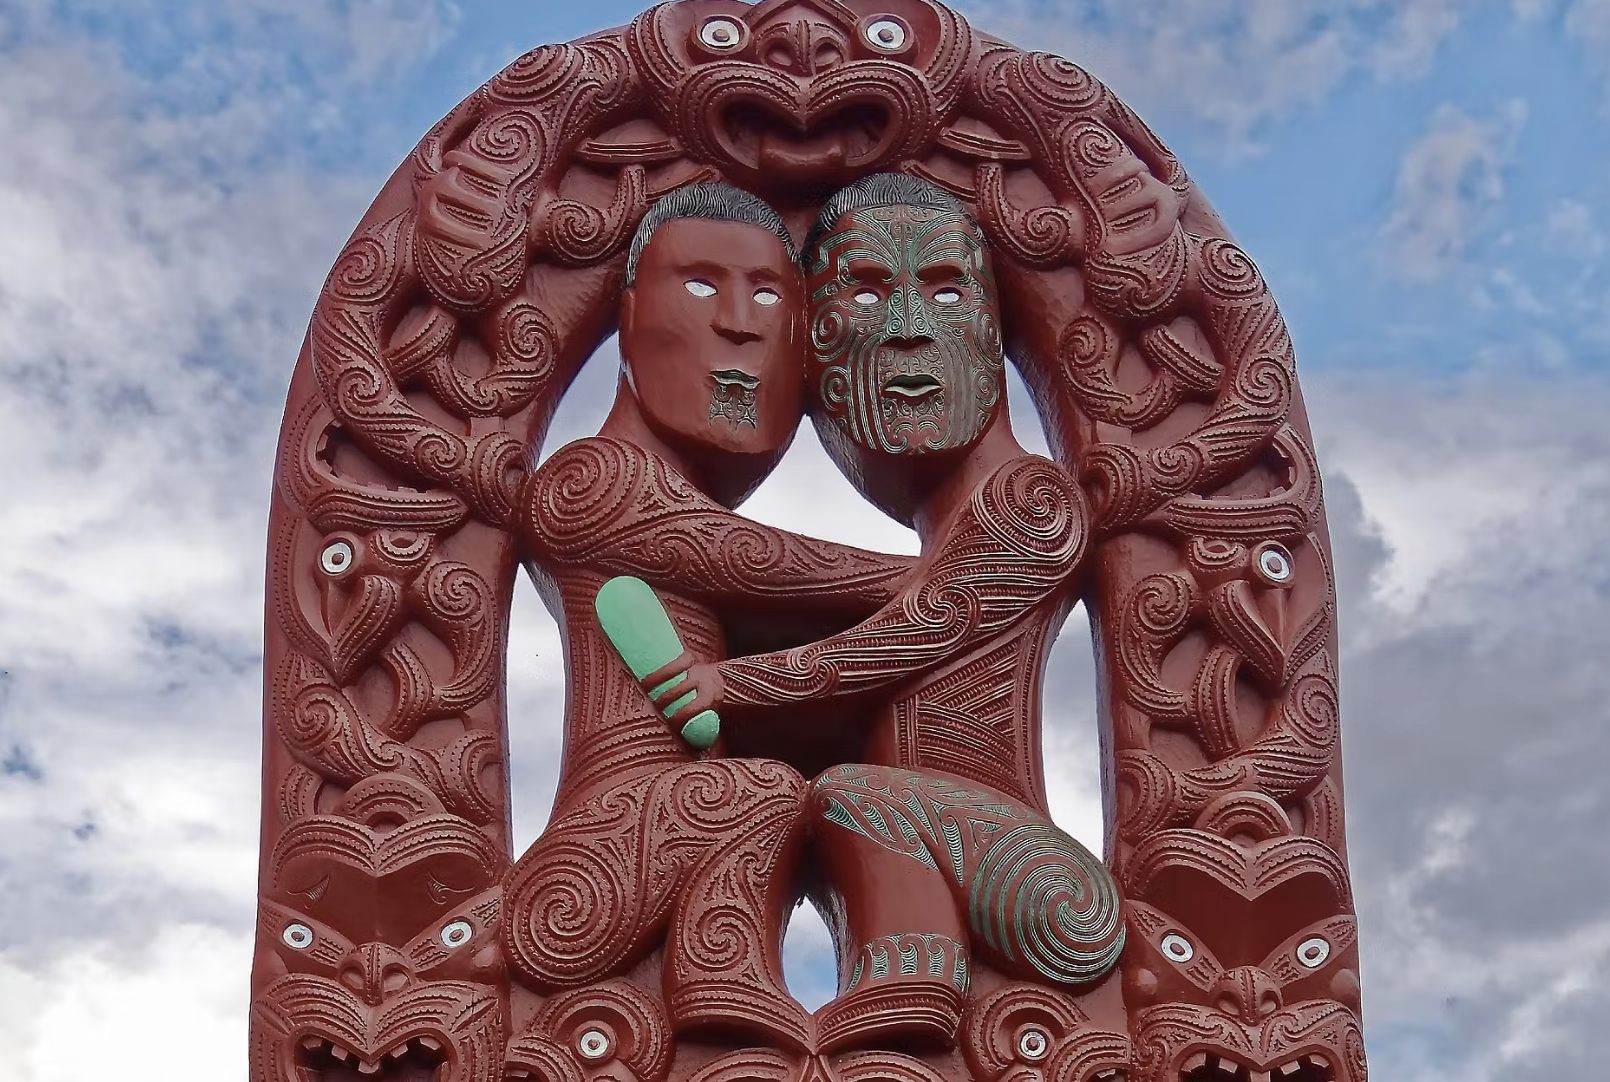
\includegraphics[width=300pt]{images/M1-1.png}}
  \caption{Māori Culture}
\end{figure}

In order to promote Māori culture around the world, our project as a digital library platform will focus on presenting Māori culture based on the Māori language and supplemented by English.

\subsection{Project Objects}
The content of our project - Māori Cultural Digital Library mainly includes the following aspects, some of which can be made into electronic materials. Include: Māori language and culture Materials, Māori Arts and Crafts,Māori History and Cultural Geography.

\subsection{Project Content}
The content format of digital library is mainly based on the following formats:
E-Books, Video and audio files, Image and text documents, Interactive Applications.

\begin{figure}[htbp]
  \centerline{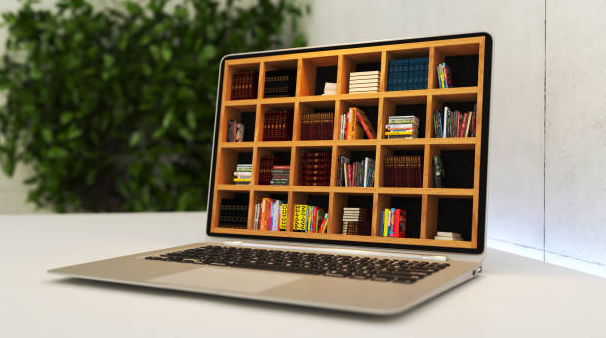
\includegraphics[width=300pt]{images/M1-2-1.png}}
  \caption{Digital Libraries}
\end{figure}

\subsection{Project Direction}
Our project can be made into a digital library of Māori culture, which aims to collect, preserve, display and disseminate the Māori cultural heritage online platform.

The Māori Cultural Library initially provides curriculum education to young people (13-18 years old). It integrates Māori language lessons into textbooks and provides a Māori language learning environment for teenagers.

Digital Collection of Māori Cultural Heritage: The Māori Cultural Digital Library collects important Māori heritage such as traditional culture, history, art and language through digital technology, forming a digital cultural database, so that more people can easily access and understand Māori culture.

Promoting the inheritance and development of Māori culture: The Digital Library of Māori Culture is not only a platform for the collection and preservation of cultural heritage, but also an important tool for promoting the inheritance and development of Māori culture. Through digital display and dissemination, more people can learn and understand Māori culture, and help Māori themselves better protect and pass on their own culture.

Providing education and research resources: The Digital Library of Māori Culture is not only a showcase, it also provides a wealth of education and research resources, so that students, teachers and researchers can understand and study Māori culture more deeply, and promote the development of Māori cultural research.

Collaboration with other cultural digital libraries: Māori cultural digital libraries can collaborate with other cultural digital libraries to share cultural resources and experiences and enhance cultural exchange and understanding. In this way, more people can know about Māori culture, and at the same time, Māori can better understand and respect other cultures.

Protecting and inheriting the sustainability of Māori Culture: The Māori Cultural Digital Library is an important tool for protecting and inheriting Māori culture, which needs to be constantly updated and improved to ensure the sustainability of Māori cultural heritage. At the same time, it is also necessary to actively participate in community cultural activities to promote the development and inheritance of Māori culture.
 
\section{Background analysis}

\subsection{Digital Library}

Digital library refers to the library that uses digital technology to store, organize, retrieve, transmit, utilize and protect document resources. Different from traditional physical libraries, digital libraries are mainly dominated by literature resources in electronic form, which can be retrieved and accessed through computer networks. Digital library is the product of the information age. It uses the digital way to manage the document resources, which makes it more convenient for people to obtain and use the information resources, and also provides a broader space for academic research and education\cite{HowtoBui15:online}.

Digital library is of great significance to academic research and education. It provides more extensive and deeper information resources for education and research, and provides a more convenient and efficient learning, research and teaching platform for scholars, researchers and students. At the same time, digital library also provides a wider range of cultural and knowledge resources for the society, and promotes cultural exchange and knowledge innovation.

\begin{figure}[htbp]
  \centerline{
\includegraphics[width=300pt]{images/M1-2-2.png}}
  \caption{Books about Digital Libraries}
\end{figure}

\subsection{Main Features}
The main features of a digital library include:
Electronic resources, Resource sharing, Search function, Knowledge management, Globally, etc\cite{Internat75:online}.

\subsection{Content}
In general, digital library includes literature resources, metadata, search tools, digital library systems, services and support, and rights management. These contents together constitute the basic elements of digital library, providing users with convenient, fast and efficient information resources services.
Literature resources,Metadata,Search tools, Digital library system, Services and Support, Copyright Management.

\subsection{Usage}
In order to give full play to the role of digital library, enterprises should ensure the effective protection of information retrieval, knowledge management, training and education after the establishment of digital library system. Enterprises also need to be equipped with special digital library administrators, responsible for the maintenance and update of digital library, to ensure that the resources and functions of digital library always keep the latest, the most comprehensive, the most valuable.

\subsection{Cost}
In general, most of the cost of digital library lies in the establishment and maintenance. However, the advantage of digital library is that it can greatly save the storage space and maintenance cost of traditional library, and digital library can provide richer and more convenient resources and services to bring better experience for users.
 


\chapter{Comparative study and analysis}

\section*{Introduction}

\lettrine[lines=2]{A}\\s In order to achieve the objectives of the project, Group 2 researched some of the typical platforms that are currently popular in the industry and analysed their main features, with the aim of incorporating their strengths in the project. Popular software used for the development of digital library systems and platforms include Greenstone, Dspace, Invenio, Omeka S, EPrints, Mukurtu.

\section{Key Features of typical platforms}

\subsection{Greenstone}

Greenstone is basically a relatively complete open source software to meet the needs of the general digital library, but also very suitable for newcomers to start. Its main features are support for multiple languages, multiple digital material formats and cross-platform. greenstone can run on multiple operating systems, including Windows, Mac OS X, Linux, etc. In addition, greenstone supports a variety of open standards and protocols, such as OAI-PMH, Dublin Core, MARC, etc., can Easily integrate digital libraries and web publications with other systems.



\subsection{Dspace}

DSpace is an open source digital repository software, the main features of DSpace are its security and community support, DSpace provides a complete permission management system that helps users control who can access and edit the content in the repository while keeping the content secure. 

\begin{figure}[htbp]
  \centerline{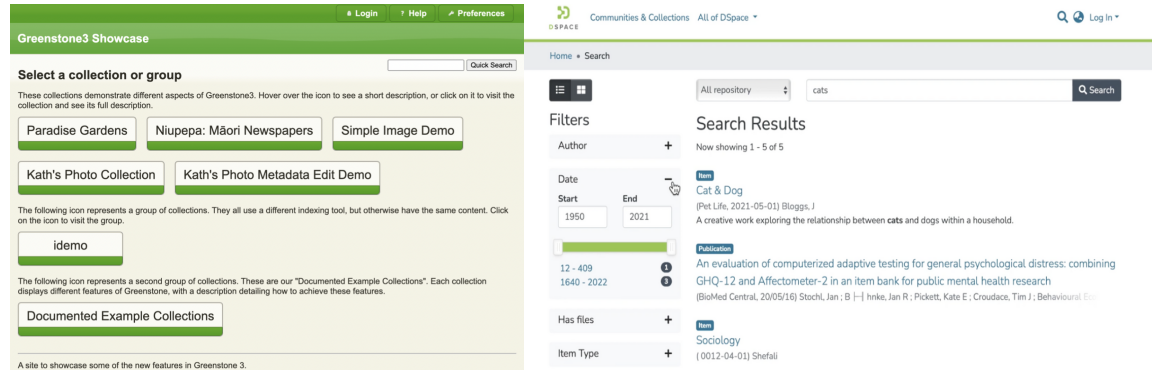
\includegraphics[width=500pt]{images/a1.jpg}}
  \caption{Greenstone \& DSpace}
\end{figure}

\subsection{Invenio}

Invenio is a framework and not a repository software delivered directly. So it requires developers to develop code to refine the implementation of their own platform. Its main features are the powerful search functionality and the ability to handle data storage. It uses all the features of Elasticsearch.



\subsection{Omeka S}
It is a free, open source web application for creating and managing digital documents and online exhibitions.The main feature of Omeka S is the customisable exhibition functionality, with custom exhibition settings based on user needs and support for a wide range of exhibition templates and themes.

\begin{figure}[htbp]
  \centerline{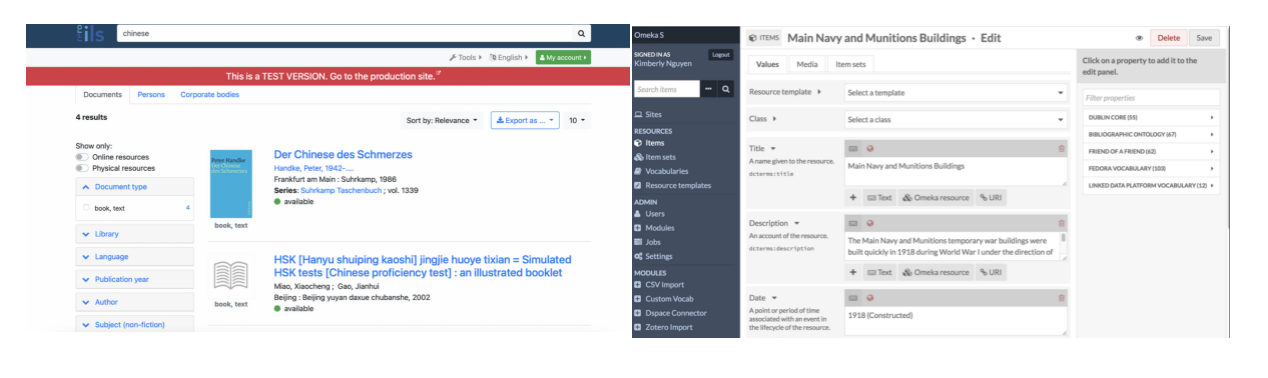
\includegraphics[width=500pt]{images/a9.jpg}}
  \caption{Invenio \& Omeka S}
\end{figure}

\subsection{EPrints}
The main features of EPrints are its support for a wide range of metadata standards and its statistical and analytical functions. It supports a wide range of metadata standards to facilitate the input and output of data. In addition, its statistical and analytical features help users to understand the usage of the digital repository, user preferences for resources, etc.


\subsection{Mukurtu}
Mukurtu is an open source digital library and community framework. Its most important feature is that it provides a way of managing cultural heritage that can help preserve and pass on the heritage of a culture. mukurtu's emphasis on community collaboration allows community members to participate in the management and sharing of cultural heritage. In addition, Mukurtu supports the creation and management of cultural protocols, allowing cultural heritage to be managed and shared in accordance with the traditional cultural protocols and norms of the community. This feature allows for the conservation of cultural heritage and the interchange of cultures within the project.


\begin{figure}[htbp]
  \centerline{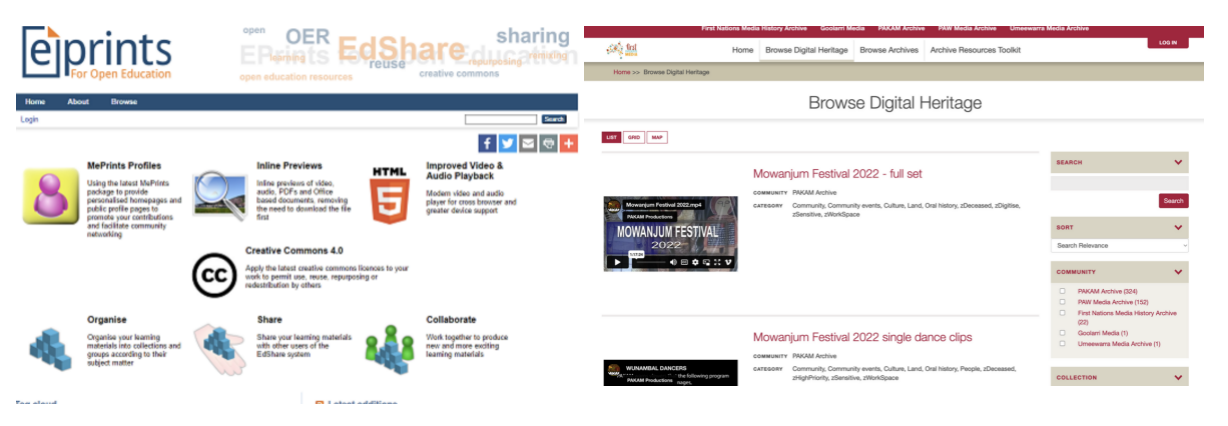
\includegraphics[width=500pt]{images/a8.jpg}}
  \caption{EPrints \& Mukurtu}
\end{figure}


\section{Comparison Chart}
Group 2 has selected a few key attributes that need to be met in a project, comparing the six popular open source software for creating digital libraries mentioned above and creating the following comparison chart. These key attributes can be used to target the advantages of some platforms into our projects.

\begin{figure}[htbp]
  \centerline{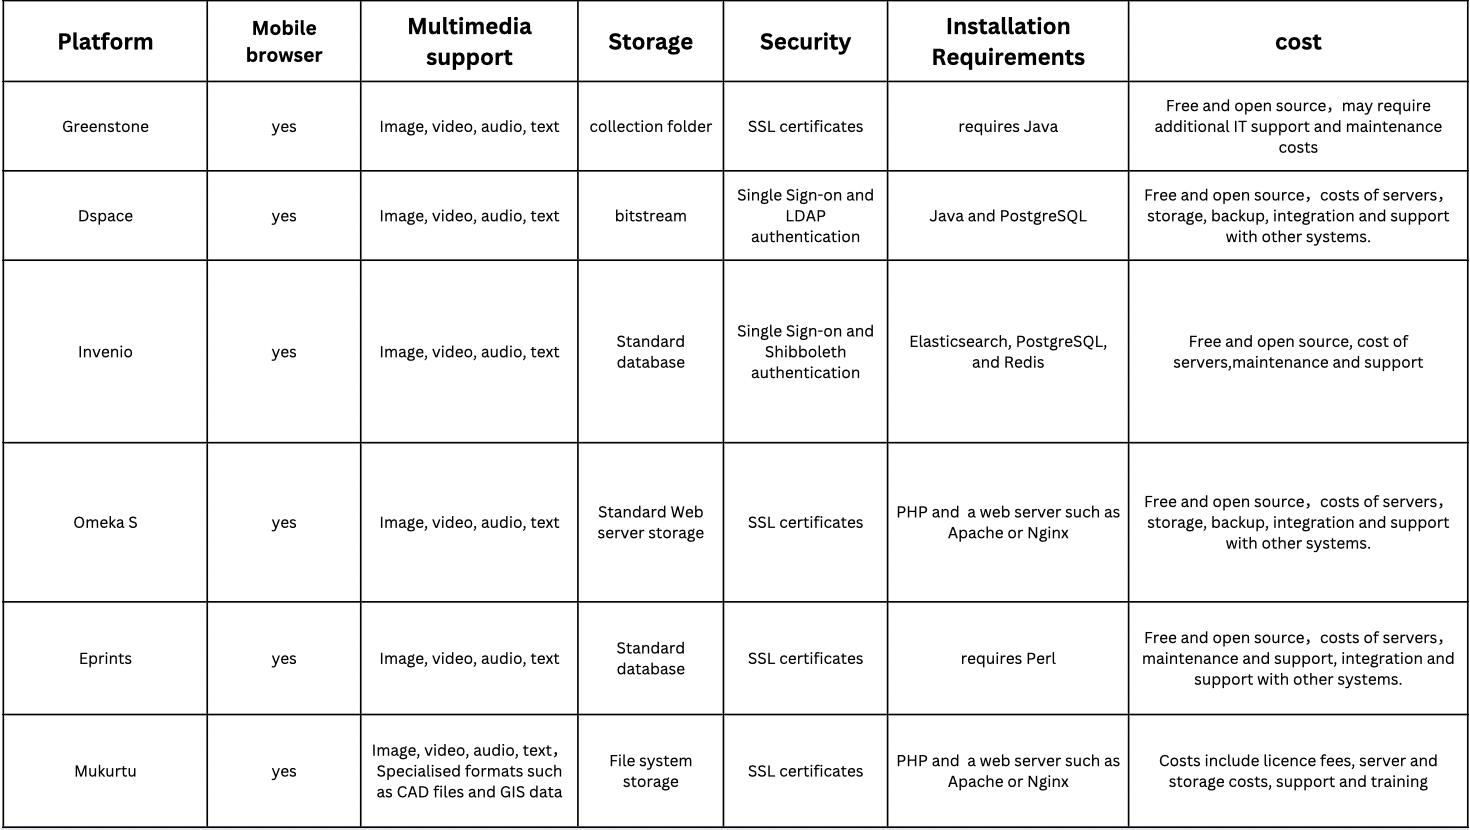
\includegraphics[width=500pt]{images/a2-1.jpg}}
  \caption{Comparison Chart}
\end{figure}


\section{Conclusion}
The main features of six popular open source software for creating digital libraries were analysed through a study of their main features, and according to the requirements of the project, to achieve the transmission and preservation of Māori culture, there was also a need to provide a platform space to allow cultural exchange between members. These requirements are the main aims that need to be achieved. But for the essence of the platform such as data security, multimedia files, cost etc. these are the factors that need to be considered. It is possible to combine the different characteristics of the above platforms and incorporate their main strengths to create the project.


 
\chapter{Prototype Design}

The aim of this project is to design and develop a prototype digital library for Māori language users to meet the needs of Māori language users for book retrieval, borrowing and return functions, and to improve the library experience for Māori language users. The prototype library is aimed at the Maori speaking community around the world, including Maori teachers, students, parents and general users\cite{Pixso0:online}.

Māori language is one of the official languages of New Zealand's indigenous Maori people and is an important part of New Zealand's cultural and social development. In order to promote the heritage and development of the Maori language, the prototype digital library will provide Maori language users with rich and diverse Maori language book resources to facilitate their online reading and learning, and will also make a positive contribution to Maori language education and cultural heritage\cite{Discover30:online}.

\section{Design principles and methodology}

The design of the digital library prototype will follow the following principles:

User-centered: The project will focus on user needs, user experience and satisfaction, to provide users with efficient and convenient humanized services.

Diversity and inclusion: The digital library prototype will provide a variety of resources from the rich and diverse Māori language culture, covering different areas and topics, embracing a variety of cultures and ideologies, and reflecting the diversity of Māori culture.

\section{Prototype introduction}

\subsection{Main interface}

\begin{figure}[htbp]
  \centerline{
\includegraphics[width=400pt]{images/3-1-1.png}}
  \caption{Main interface}
  \label{fig30}
\end{figure}

After the user logs in, the main interface will show the Māori cultural background, the address of the Maori cultural community, the pictures of the introduction of Maori cultural activities, the links of E-books and multimedia, and the search function of the whole network. Here you can find all the resources we upload and provide, and you can also ask for help to carry out Māori language practice in the community and communicate with other Maori language learners.

\subsection{User interface}

\begin{figure}[htbp]
  \centerline{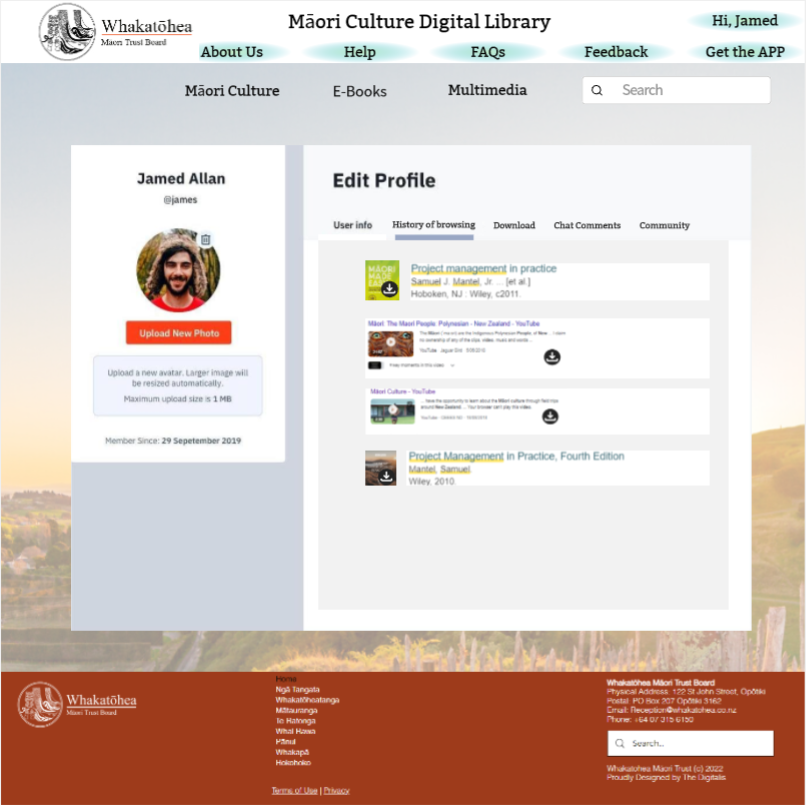
\includegraphics[width=400pt]{images/3-1-2.png}}
  \caption{User interface}
  \label{fig30}
\end{figure}

After the user logs in, The system will record user information, users can modify information through the user interface, view browsing history and like the collection of E-books or multimedia, also can communicate with friends here and view the comments of E-books or multimedia.

\subsection{Māori cultural interface}

\begin{figure}[htbp]
  \centerline{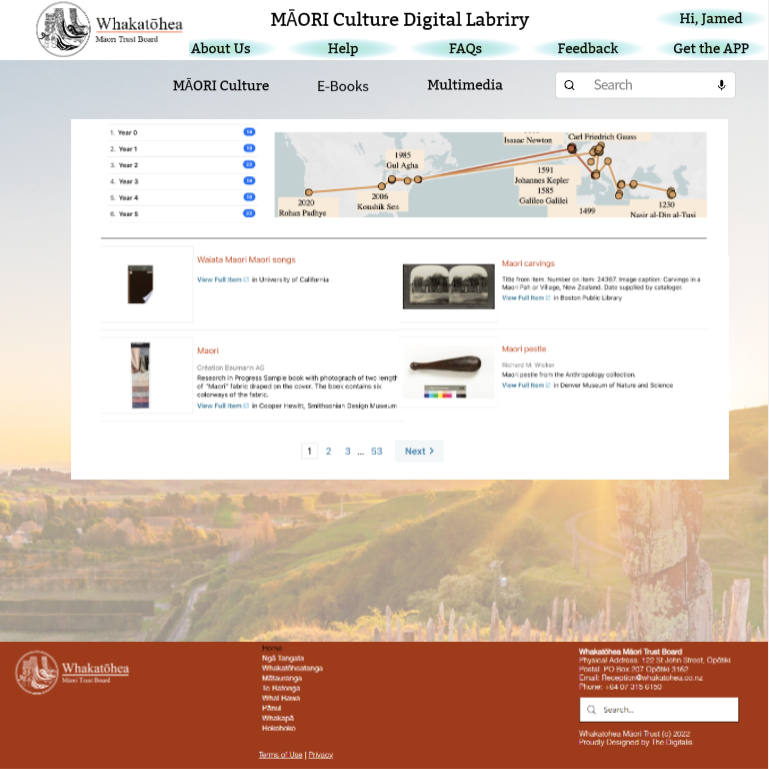
\includegraphics[width=400pt]{images/3-1-3.png}}
  \caption{Māori cultural interface}
  \label{fig30}
\end{figure}

We add a Māori culture interface where users can find all about the development process of Māori culture, migration history and distribution changes, as well as the existing Māori cultural products, which will provide more research channels for current and future learners of Māori culture, from buildings, objects to custom products to show the development process of Māori culture in all aspects\cite{MāoriCul4:online}.

\subsection{E-books browsing interface}

\begin{figure}[htbp]
  \centerline{
\includegraphics[width=400pt]{images/3-2-1.png}}
  \caption{E-books browsing interface}
  \label{fig30}
\end{figure}

In the E-books browsing interface, users can search related E-books through filters, and all filters we designed include the function of voice input, which can provide convenience for some disabled learners. Typing a keyword in the filter or filtering in the left toolbar will display the relevant E-books.

\subsection{The E-book interface}

\begin{figure}[htbp]
  \centerline{
\includegraphics[width=400pt]{images/3-2-2.png}}
  \caption{The E-book interface}
  \label{fig30}
\end{figure}

In the E-books interface, users can read text or listen to E-books through the voice playback function, and provide translation functions for other languages. All resources provided by the e-library are downloadable.

\subsection{Video interface}

\begin{figure}[htbp]
  \centerline{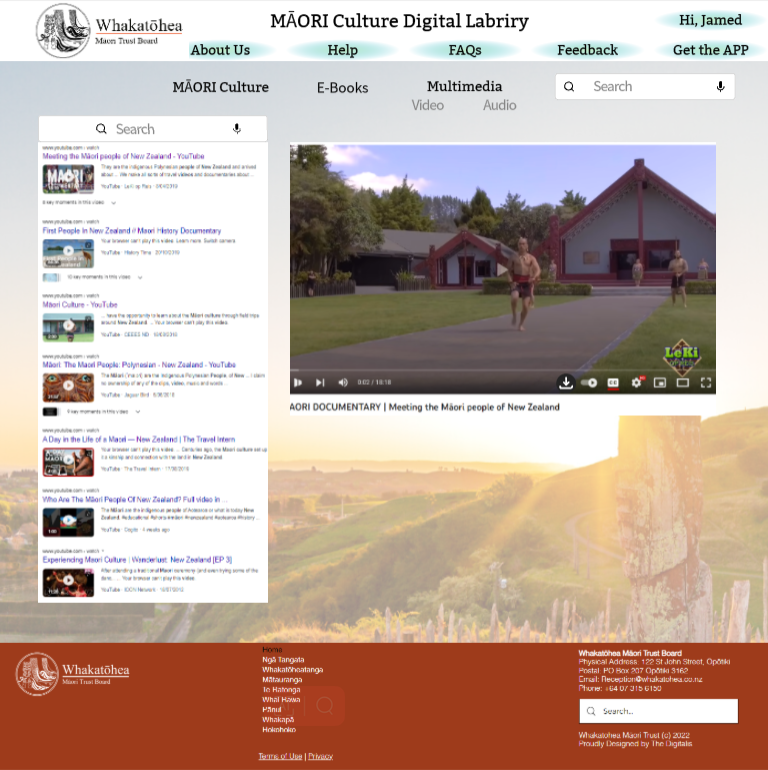
\includegraphics[width=400pt]{images/3-3-1.png}}
  \caption{Video interface}
  \label{fig30}
\end{figure}

In the video interface, users can search related videos by keywords or related words. The filter provides many options such as upload time, picture quality, video duration, and subtitles in other language to facilitate Māori learners to view.

\subsection{Audio interface}

\begin{figure}[htbp]
  \centerline{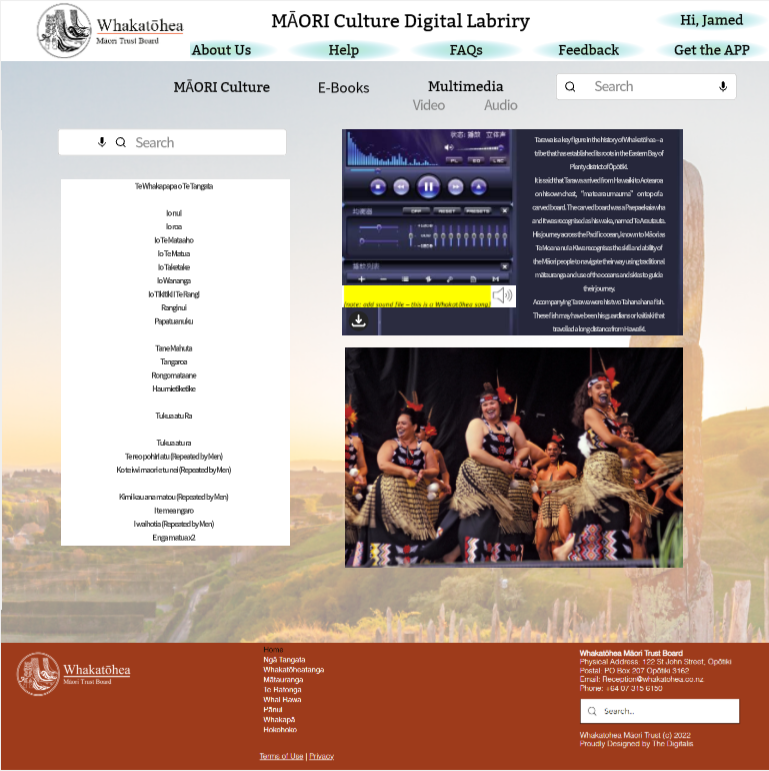
\includegraphics[width=400pt]{images/3-3-2.png}}
  \caption{Audio interface}
  \label{fig30}
\end{figure}

In the audio interface, users can search related audio by the keywords or related words. When playing audio files, subtitles in other languages will be displayed synchronously in the player, and the audio content will be displayed on the left side, which can provide learning convenience for Māori language learners. Audio related videos or pictures are displayed below, which provides a good learning environment for audio learning and deefies learners' memory\cite{MaoriHis64:online}.

\section{Conclusion and Prospect}

Through the design and implementation of this project, the prototype of digital library for Maori users has realized the main functions such as book and multimedia retrieval. The library prototype can provide rich and diverse Maori cultural resources to facilitate users to read and learn online\cite{Māori–Te85:online}.

The designed prototype still has some limitations and shortcomings, including the process of user interface design and interaction can be further optimized, the function of multimedia interface can be more humanized, and the front-end visualization of the library can be more abundant to meet all Maori culture learners for learning.

As technology continues to advance and the Maori language community continues to grow, the digital library prototype needs to be constantly updated and upgraded to meet the changing needs and expectations of its users. At the same time, the digital library will also make greater contributions to the Maori language education and cultural inheritance, promote the inheritance and development of the Maori language, and promote the communication and integration of multiple cultures. We look forward to the Maori Digital library becoming an important learning and communication platform for Maori language users and making greater contributions to the future development of the Maori language community\cite{MaoriCul16:online}.


\chapter{Feedbacks}
\chaptermark{Feedbacks}
Based on the feedback from the previous presentation, we initially had a prototype with only text input for the search function. However, considering the specific needs of some users and the functionality of search, we added a voice input feature for searching. We also implemented a pop-up window for converting voice to text. Additionally, we lacked details on accessing ebooks in our original model, so we added a download ebooks feature in the download list for users to view and download ebooks at any time. Furthermore, we recognized the need for user interaction with the digital library and to achieve our goal of promoting indigenous culture. Hence, we included community interaction and quizzes to enhance user engagement.


\chapter{Conclusion\&next steps} 
\chaptermark{Conclusion\&next steps}

We have currently achieved the basic integration of the frontend and backend models, which can adequately fulfill the usage and development of a digital library platform. In the future, there may be design enhancements to the user interface to engage the interest of young users. However, our initial goal for creating the digital library was to target teenagers, and subsequent improvements may be best suited for the general public. This will facilitate the increasing number of people learning about tribal culture.




% \bibliographystyle{plain}
% \bibliography{biblio}
\printbibliography
\end{document} 